\section{Paraboloide}
Vi vil nu undersøge den geodætiske kurve på en paraboloide, der ser således ud: \\
$$F(x,y)=(x,y,\frac{1}{2}(x^2+y^2))$$ \\
Man kunne finde den geodætiske kurve på formen $(x,y)->(cos(\phi)*r(\phi),sin(\phi)*r(\phi))$. I såfald vil Lagrange-funktionen se således ud: \\
$$L = \int_{a}^{b}\sqrt{(\frac{d}{d\phi}(cos(\phi)r(\phi)))^2+(\frac{d}{d\phi}(sin(\phi)r(\phi)))^2+(\frac{d}{d\phi}((cos(\phi)r(\phi))^2+(sin(\phi)r(\phi))^2))^2}dt = \sqrt{\dot{r}^2+r^2+\dot{r}^2r^2}$$
Vores ligning hedder $\frac{\partial L}{\partial r}-\frac{d}{dt}\frac{\partial L}{\partial \dot{r}}$ og der sættes ind: \\
$$\frac{\partial L}{\partial r}-\frac{d}{dt}\frac{\partial L}{\partial \dot{r}}=\frac{r+r\dot{r}^2}{\sqrt{\dot{r}^2+r^2+\dot{r}^2r^2}}-\frac{r(-\dot{r}^2+\dot{r}^4+r^2\dot{r}^2+r^2\dot{r}^4+r\ddot{r}+r^3\ddot{r})}{(\dot{r}^2+r^2+\dot{r}^2r^2)^\frac{3}{2}}=\frac{r(2\dot{r}^2+r^2+r^2\dot{r}^2-r\ddot{r}-r^3\ddot{r})}{(\dot{r}^2+r^2+\dot{r}^2r^2)^\frac{3}{2}}=0$$ \\
Dette giver differentialligningen: \\
$$r(2\dot{r}^2+r^2+r^2\dot{r}^2-r\ddot{r}-r^3\ddot{r})=0$$ \\
Det er en andenordens differentialligning som ikke er lineær. Denne lader sig heller ikke løse analytisk, så den må løses numerisk. Vi har valgt at løse ligningen for værdier for $\phi$ på 1 og 3. Dette giver kurven:\\
\begin{figure}[h]
\caption{Den grønne linje er geodæten, og den sorte er den lige linje i (x,y)-planen}
\centering
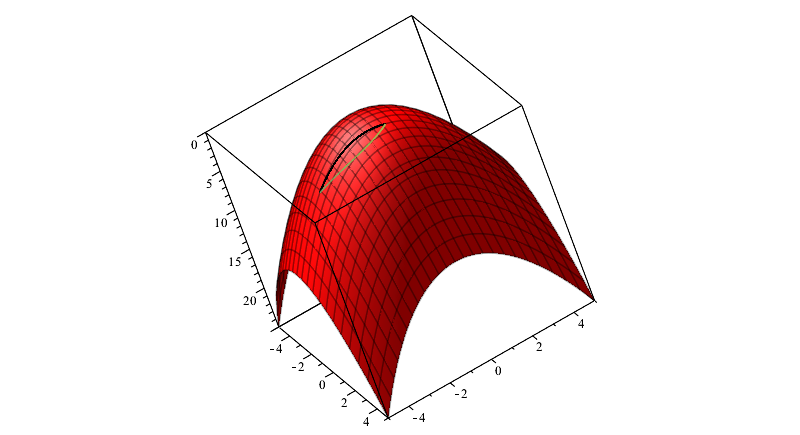
\includegraphics[scale=0.4]{paracurolineny}
\end{figure}
\\
Ved udregning af længderne er vores geodæt også den korteste, da den har en længde på 3,2 mens den lige linje har en længde på 4,7.